\section{Évaluation de l'hypothèse de rentabilité}
\label{section:4.5-HYPOTHESE-RENTABILITE}

	%%% Introduction / Transition.
	Dans les études précédentes, le cas d'arrêt de notre méthodologie d'annotation basée sur le \textit{clustering} interactif était conditionné à la vérité terrain.
	En effet, nous utilisions un seuil de $90$\% de \texttt{v-measure}, caractérisant une annotation dite "partielle" de la base d'apprentissage.
	Cependant, une telle référence n'est pas accessible en situation réelle car l'objectif de notre méthode est précisément de la construire cette vérité terrain.
	Nous devons donc nous intéresser à d'autres moyens pour estimer la rentabilité d'une itération supplémentaire et pouvoir ainsi définir de nouveaux cas d'arrêt pour le \textit{clustering} interactif.
	Pour cela, nous aimerions vérifier l'hypothèse suivante :
	
	%%% Formulation des hypothèses:
	\begin{tcolorbox}[
		title=\faVial~\textbf{Hypothèse de rentabilité}~\faVial,
		colback=colorTcolorboxHypothesis!15,
		colframe=colorTcolorboxHypothesis!75,
		width=\linewidth
	]
		« \textbf{
			Au cours d'une méthodologie d'annotation basée sur le \textit{clustering} interactif, il est possible d'estimer la rentabilité d'une itération supplémentaire de la méthode, et ainsi d'établir des cas d'arrêt indépendant d'une vérité terrain pour obtenir une base d’apprentissage satisfaisante.
		} » \\
		
		% Figure.
		La \textsc{Figure~\ref{figure:4.5-HYPOTHESE-RENTABILITE}} illustre cette hypothèse et l'espoir de pouvoir estimer le rapport entre le gain de pertinence obtenu et le coût nécessaire pour l'obtenir.
		%
		\begin{figure}[H]  % keep [H] to be in the tcolorbox.
			\centering
			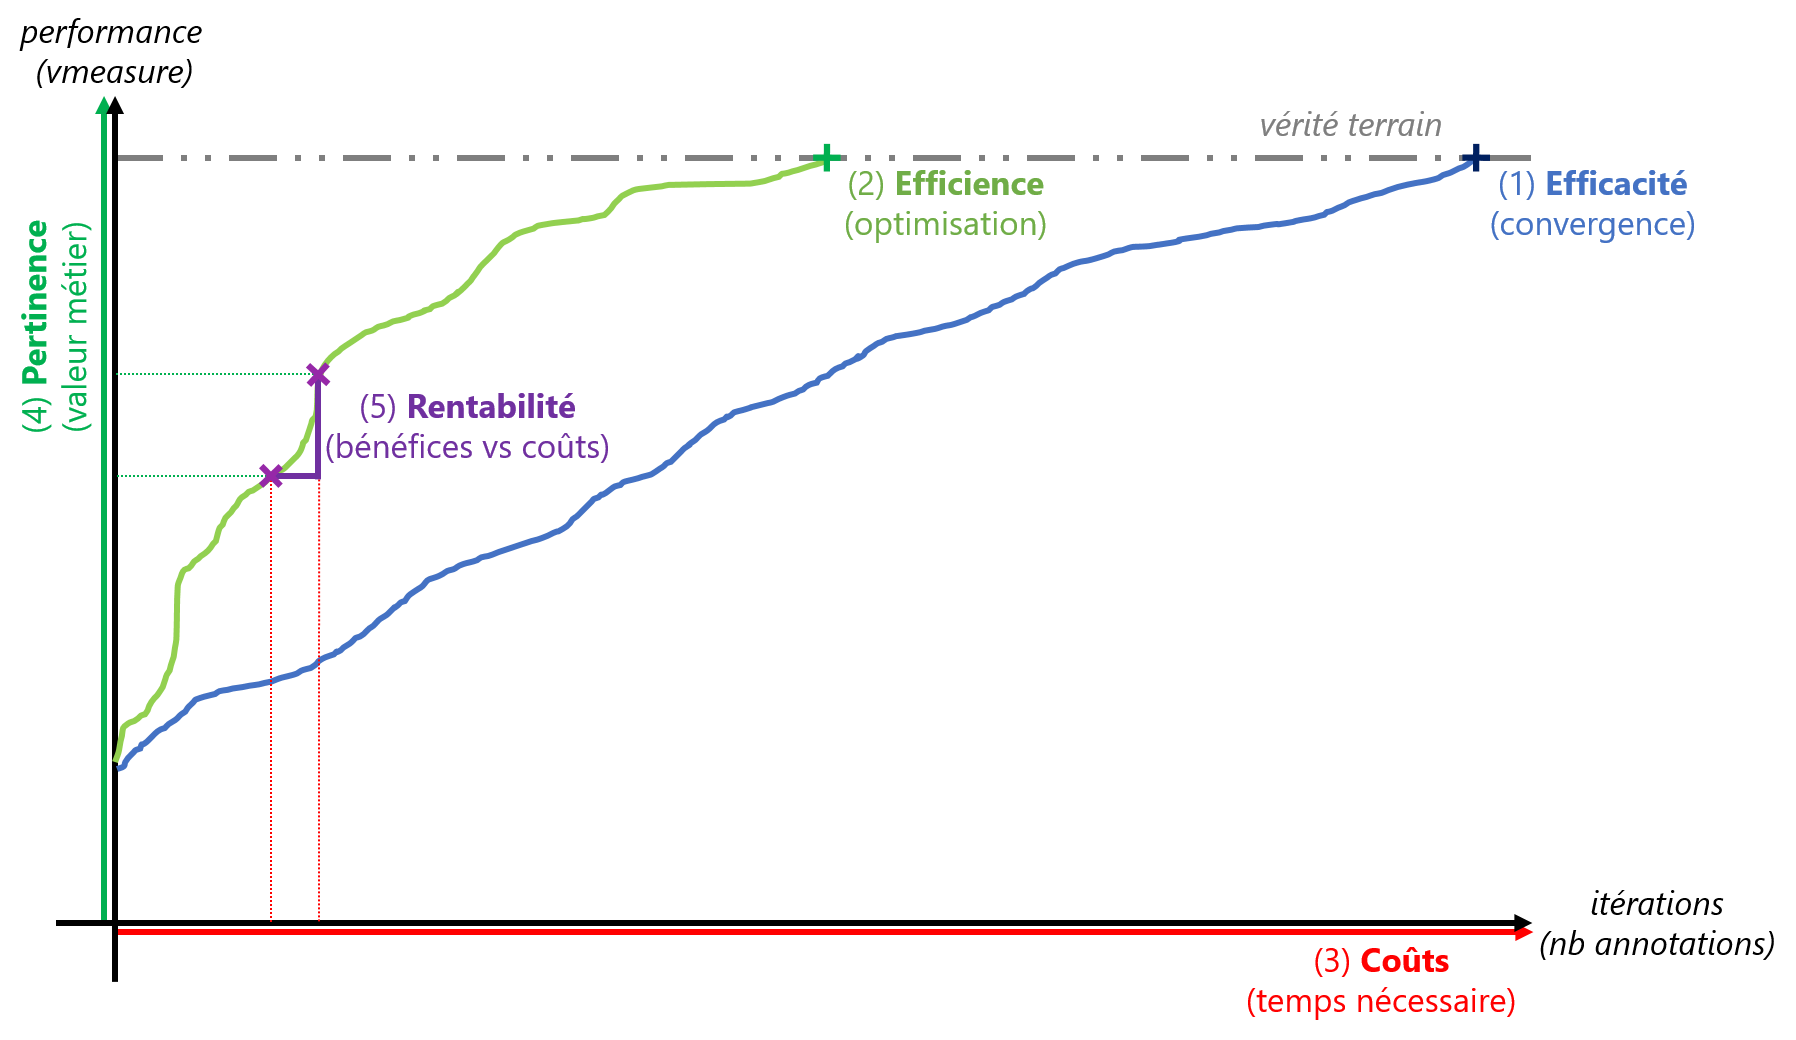
\includegraphics[width=0.95\textwidth]{figures/hypotheses-05-rentabilite}
			\caption{Illustration des études réalisées sur le \textit{clustering} interactif (\textit{étape 5/6}) en schématisant l'évolution de la pertinence (\textit{valeur métier évaluée par l'expert et exprimé en nombre de clusters}) d'une base d'apprentissage en cours de construction en fonction du coût temporel de la méthode (\textit{temps nécessaire à l'expert métier et à la machine}), ainsi que la rentabilité de chaque itération de la méthode (\textit{rapport entre le gain potentiel de pertinence et le coût à investir}).}
			\label{figure:4.5-HYPOTHESE-RENTABILITE}
		\end{figure}

	\end{tcolorbox}
		
	% Résumé de l'étude.
	Afin de vérifier cette hypothèse, nous explorons deux approches :
	\begin{itemize}
		\item l'évolution de l'\textbf{accord entre l'annotation de l'expert et le \textit{clustering}} sur lequel est basé l'échantillon d'annotation, permettant d'estimer si la machine doit encore être corrigée par l'annotateur  (cf. \textsc{Section~\ref{section:4.5.1-ETUDE-RENTABILITE-ACCORD-ANNOTATION-CLUSTERING}}) ;
		\item et l'évolution de la \textbf{différence entre deux \textit{clusterings} successifs}, permettant de mesurer s'il y a eu des changements visibles dans le partitionnement des données après l'ajout des dernières contraintes (cf. \textsc{Section~\ref{section:4.5.2-ETUDE-RENTABILITE-SIMILARITE-CLUSTERING}}).
	\end{itemize}
	
	
	%%%
	%%% Subsection 4.5.1: Étude de l'évolution d'accord entre l'annotation et le \textit{clustering}.
	%%%
	\subsection{Étude de l'évolution d'accord entre l'annotation et le \textit{clustering}}
	\label{section:4.5.1-ETUDE-RENTABILITE-ACCORD-ANNOTATION-CLUSTERING}
		
		% Objectif de l'expérience.
		Nous cherchons à trouver un cas d'arrêt du \textit{clustering} interactif ne nécessitant pas de comparaison avec une vérité terrain, et notre première intuition concerne l'étude des annotations réalisées.
		En effet, à chaque itération, l'expert annote un échantillon de contraintes dans le but de confirmer ou de corriger le \textit{clustering} de l'itération précédente.
		Or, après un nombre suffisant d'itérations, le \textit{clustering} commence à se stabiliser : il devrait donc y avoir davantage d’annotations qui confirment le \textit{clustering} que d'annotations qui le corrigent.
		Ainsi, nous allons étudier l'évolution du nombre de contraintes annotées qui sont en accord avec le partitionnement des données obtenu et essayer d'adapter cette analyse en cas d'arrêt pour notre méthode d'annotation.
	
		%%% Protocole expérimental.
		\subsubsection{Protocole expérimental}
			
			% Axiome.
			\begin{leftBarWarning}
				Dans le cadre de cette étude, nous supposons que l'expert métier connaît parfaitement le domaine traité dans ce jeu de données, et qu'il est capable de caractériser sans ambiguïté la similitude entre deux données issues de cet ensemble.
			\end{leftBarWarning}
			
			% Pseudo-code.
			Pour résumer le protocole expérimental que nous décrivons ci-dessous, vous pouvez vous référer au pseudo-code décrit dans \textsc{Algorithme~\ref{algorithm:4.5.1-ETUDE-RENTABILITE-ACCORD-ANNOTATION-CLUSTERING-PROTOCOLE}}.
			
			\begin{algorithm}
				\KwData{jeu de données annotés (vérité terrain)}
				%
				\ForEach{jeux de données à tester}{
					\textbf{initialisation (données)}: récupérer les données et la vérité terrain \;
					\textbf{initialisation (contraintes)}: créer une liste vide de contraintes \;
					\textbf{prétraitement}: supprimer le bruit dans les données avec \texttt{prep.simple} \;
					\textbf{vectorisation}: transformer les données en vecteurs avec \texttt{vect.tfidf} \;
					\textbf{clustering initial}: regrouper les données par similarité avec \texttt{clust.kmeans.cop} \;
					\Repeat{annotation de toutes les contraintes possibles}{
						\textbf{échantillonnage}: sélectionner de nouvelles contraintes à annoter \;
						\textbf{simulation d'annotation}: ajouter des contraintes avec \texttt{samp.closest.diff} \;
						\textbf{estimer rentabilité}: calculer l'accord entre l'annotation et le \textit{clustering} précédent \;
						\textbf{clustering}: regrouper les données par similarité avec \texttt{clust.kmeans.cop} \;
					}
				}
				\textbf{analyse 1}: afficher l'évolution de l'accord entre annotation et \textit{clustering} \;
				\textbf{analyse 2}: calculer la corrélation entre le score d'accord et le score de performance \;
				%
				\KwResult{discussion sur la rentabilité d'après l'accord entre annotation et \textit{clustering}}
				%
				\caption{\textit{Description en pseudo-code du protocole expérimental de l'étude de l'évolution d'accord entre l'annotation et le \textit{clustering}.}}
				\label{algorithm:4.5.1-ETUDE-RENTABILITE-ACCORD-ANNOTATION-CLUSTERING-PROTOCOLE}
			\end{algorithm}
			
			% Description de la vérité terrain.
			Nous utilisons comme vérité terrain le jeu de données \texttt{Bank Cards (v1.0.0)} : ce dernier traite des demandes les plus fréquentes des clients en ce qui concerne la gestion de leur carte bancaire.
			Il est composé de $500$ questions rédigées en français et réparties en $10$ classes (\texttt{perte ou vol de carte}, \texttt{carte avalée}, \texttt{commande de carte}, ...).
			Pour plus de détails, consultez l'annexe~\ref{annex:C.1-DATASET-BANK-CARDS}.
			
			% Description des tentatives de la méthode et du calcul de rentabilité.
			Sur ce jeu de données, nous exécutons une tentative complète
			\footnote{Tentative complète : itérations d'échantillonnage, d'annotation et de \textit{clustering} jusqu'à annotation de toutes les contraintes possibles.}
			\todo{Utiliser 'footmisc' et 'footref' pour faire des notes de bas de pages communes ? ou lien vers des conclusions ?}
			de la méthode du \textit{clustering} interactif utilisant notre paramétrage favori, et cette tentative est répétée $5$ fois pour contrer les aléas statistiques des exécutions.
			À chaque itération, un lot de $50$ contraintes est sélectionné puis annotés en simulant l'action d'un expert métier.
			Nous évaluons ensuite l'accord entre ces nouvelles annotations et la proposition de partitionnement des données réalisé par le \textit{clustering} à l'itération précédente :
			\begin{itemize}
				\item il y a \textbf{accord} lorsqu'une contrainte de deux données issues d'un même \textit{cluster} est annotée \texttt{MUST-LINK}, ou lorsqu'une contrainte de deux données issues de deux \textit{clusters} différents est annotée \texttt{CANNOT-LINK} (cf. \textsc{Figure~\ref{figure:4.5.1-ETUDE-RENTABILITE-ACCORD-ANNOTATION-CLUSTERING-EXEMPLE} (1)}) ;
				\item il y a \textbf{désaccord} lorsqu'une contrainte de deux données issues d'un même \textit{cluster} est annotée \texttt{CANNOT-LINK}, ou lorsqu'une contrainte de deux données issues de deux \textit{clusters} différents est annotée \texttt{MUST-LINK} (cf. \textsc{Figure~\ref{figure:4.5.1-ETUDE-RENTABILITE-ACCORD-ANNOTATION-CLUSTERING-EXEMPLE} (2)}).
			\end{itemize}
			Nous pouvons ainsi calculer un score d'accord défini par la ratio entre le nombre d'accords et le nombre de contraintes annotées.
			Pour nous permettre de discuter de l'utilité de ce score pour prédire la stabilisation du \textit{clustering} et ainsi définir un cas d'arrêt de notre méthodologie d'annotation, nous calculons aussi le score de corrélation entre cet accord et la performance obtenu à l'aide d'une vérité terrain (la corrélation \texttt{r} de \textit{Pearson} (\cite{kirch:2008:pearson-correlation-coefficient}) est utilisée).

			\begin{figure}[!htb]
				\centering
				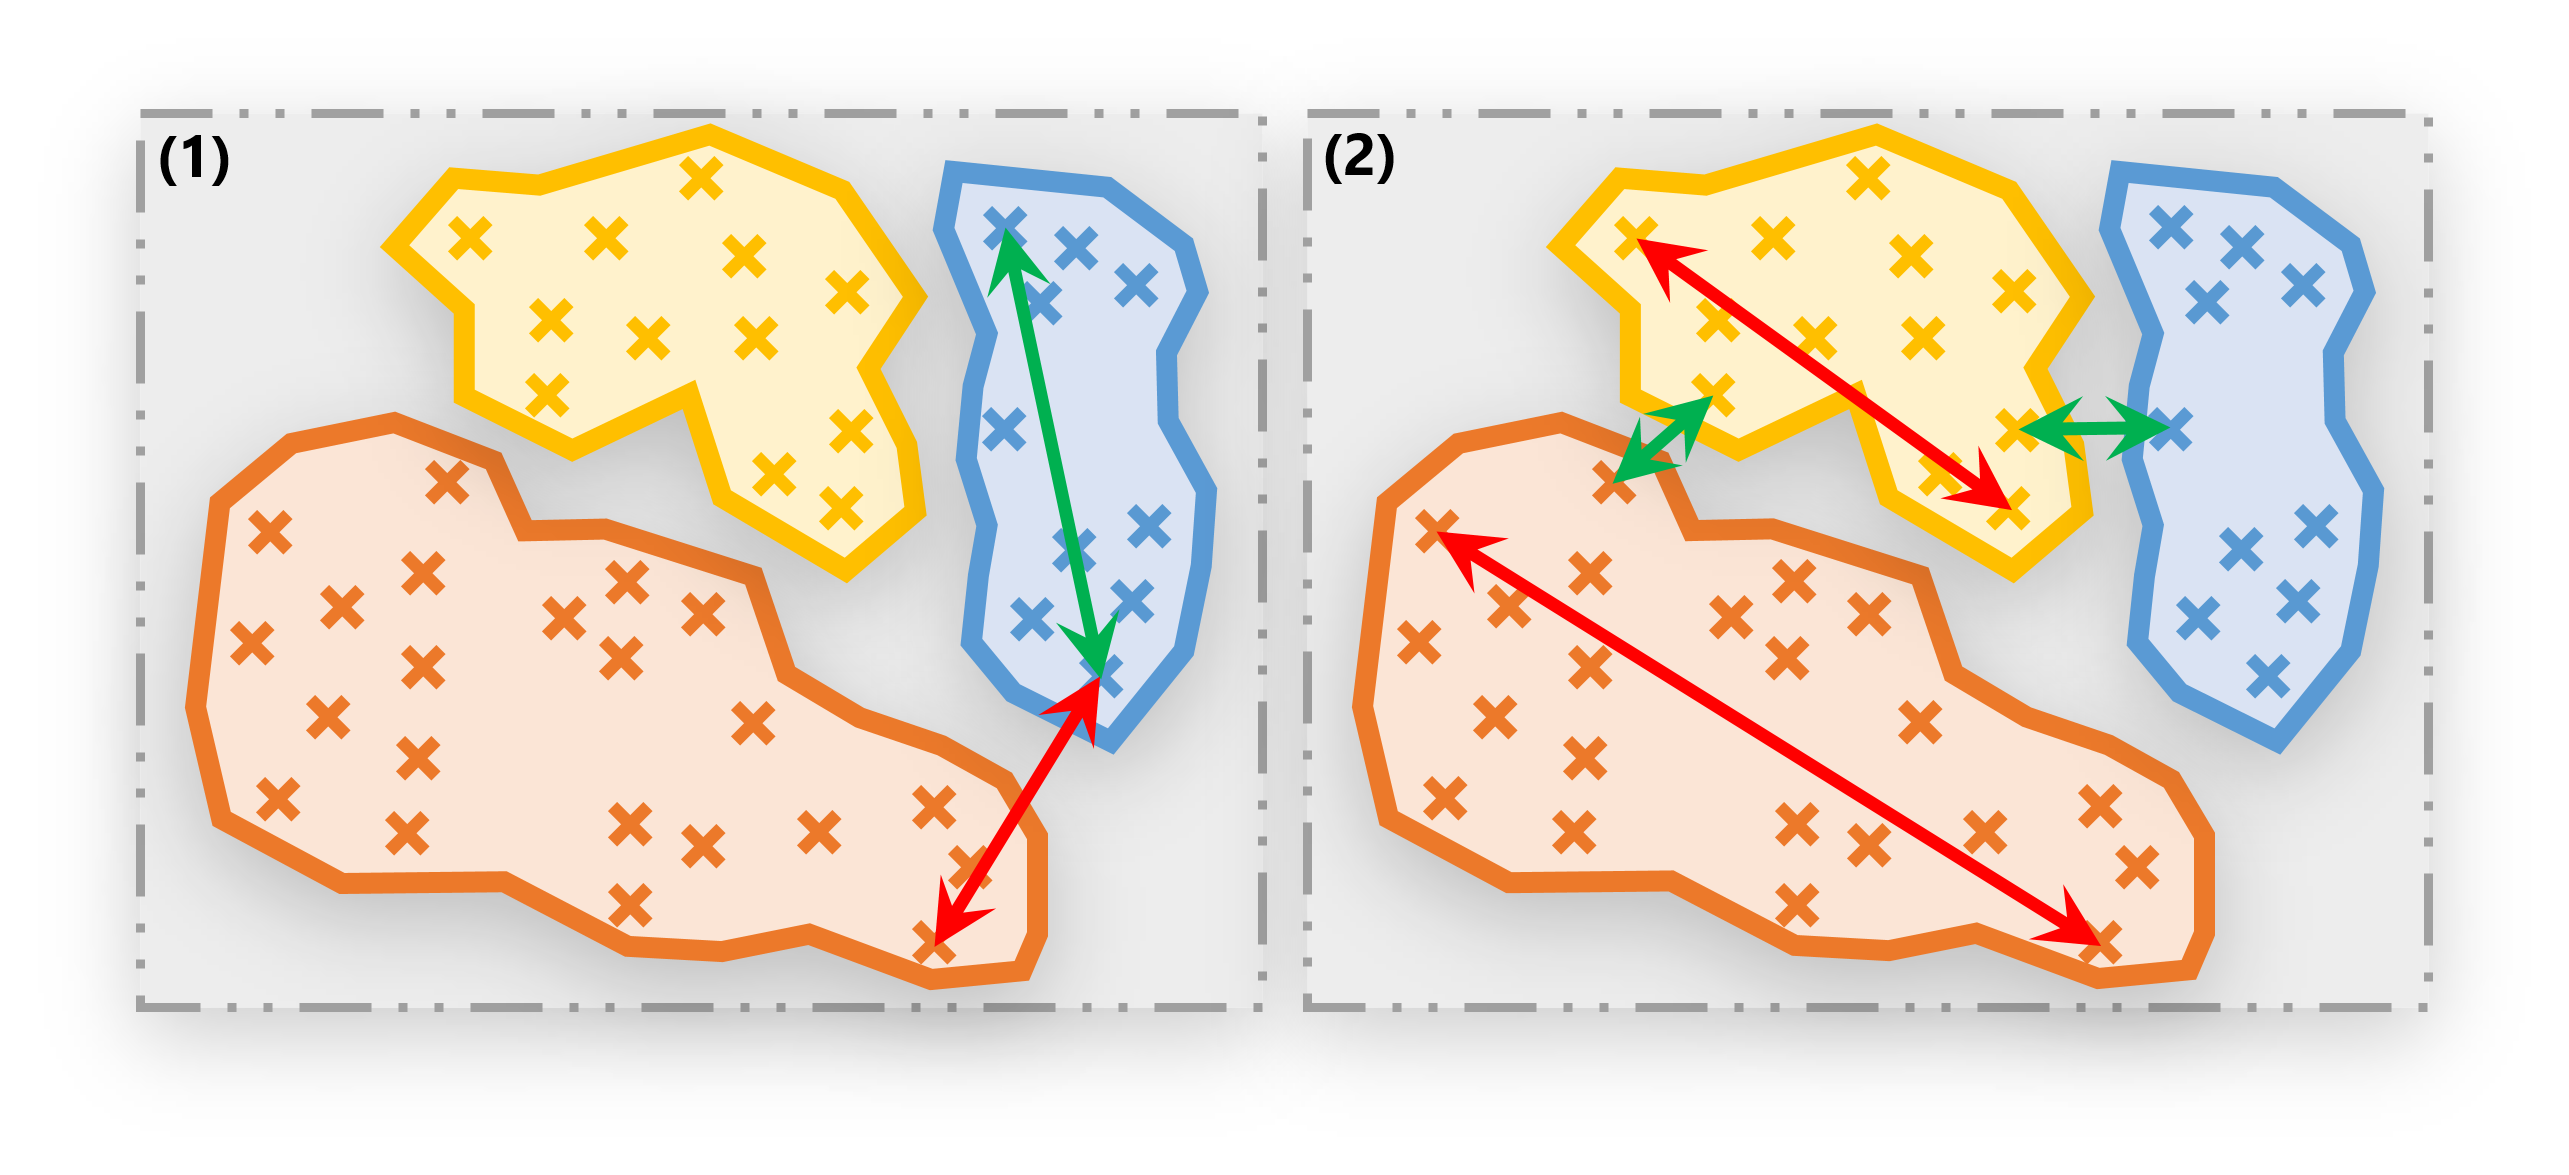
\includegraphics[width=0.7\textwidth]{figures/example-accord-annotation-clustering}
				\caption{Exemples d'accords et de désaccord entre les annotations d'une itération et le résultat du \textit{clustering} de l'itération précédente.
				Des contraintes \texttt{MUST-LINK} (flèches vertes) et \texttt{CANNOT-LINK} (flèches rouges) sont représentées dans deux situations : \textbf{(1)} montre des cas d'accords (\texttt{MUST-LINK} dans un même \textit{cluster}, \texttt{CANNOT-LINK} entre deux \textit{clusters} différents), et \textbf{(2)} montre des cas de désaccords (\texttt{MUST-LINK} entre deux \textit{clusters} différents, \texttt{CANNOT-LINK} dans un même \textit{cluster}).}
				\label{figure:4.5.1-ETUDE-RENTABILITE-ACCORD-ANNOTATION-CLUSTERING-EXEMPLE}
			\end{figure}
			
			% Référence scripts.
			\begin{leftBarInformation}
				Les scripts de l'expérience, réalisés avec des \textit{notebooks} Python (\cite{van-rossum-drake:2009:python-reference-manual}), sont disponibles dans un dossier dédié de~\cite{schild:2021:cognitivefactory-interactiveclusteringcomparativestudy}.
			\end{leftBarInformation}

		%%% Résultats
		\subsubsection{Résultats obtenus}
			
			% Figure.
			La \textsc{Figure~\ref{figure:4.5.1-ETUDE-RENTABILITE-ACCORD-ANNOTATION-CLUSTERING}} représente l'évolution moyenne du score d'accord entre annotation et \textit{clustering} pour les quatre paramétrages mis en avant lors de nos étude.
			Nous concentrons toutefois la discussion sur les résultats obtenus avec le paramétrage favori de notre méthode \textbf{(4)} et utilisons les autres résultats comme points de référence.
			\begin{figure}[!htb]
				\centering
				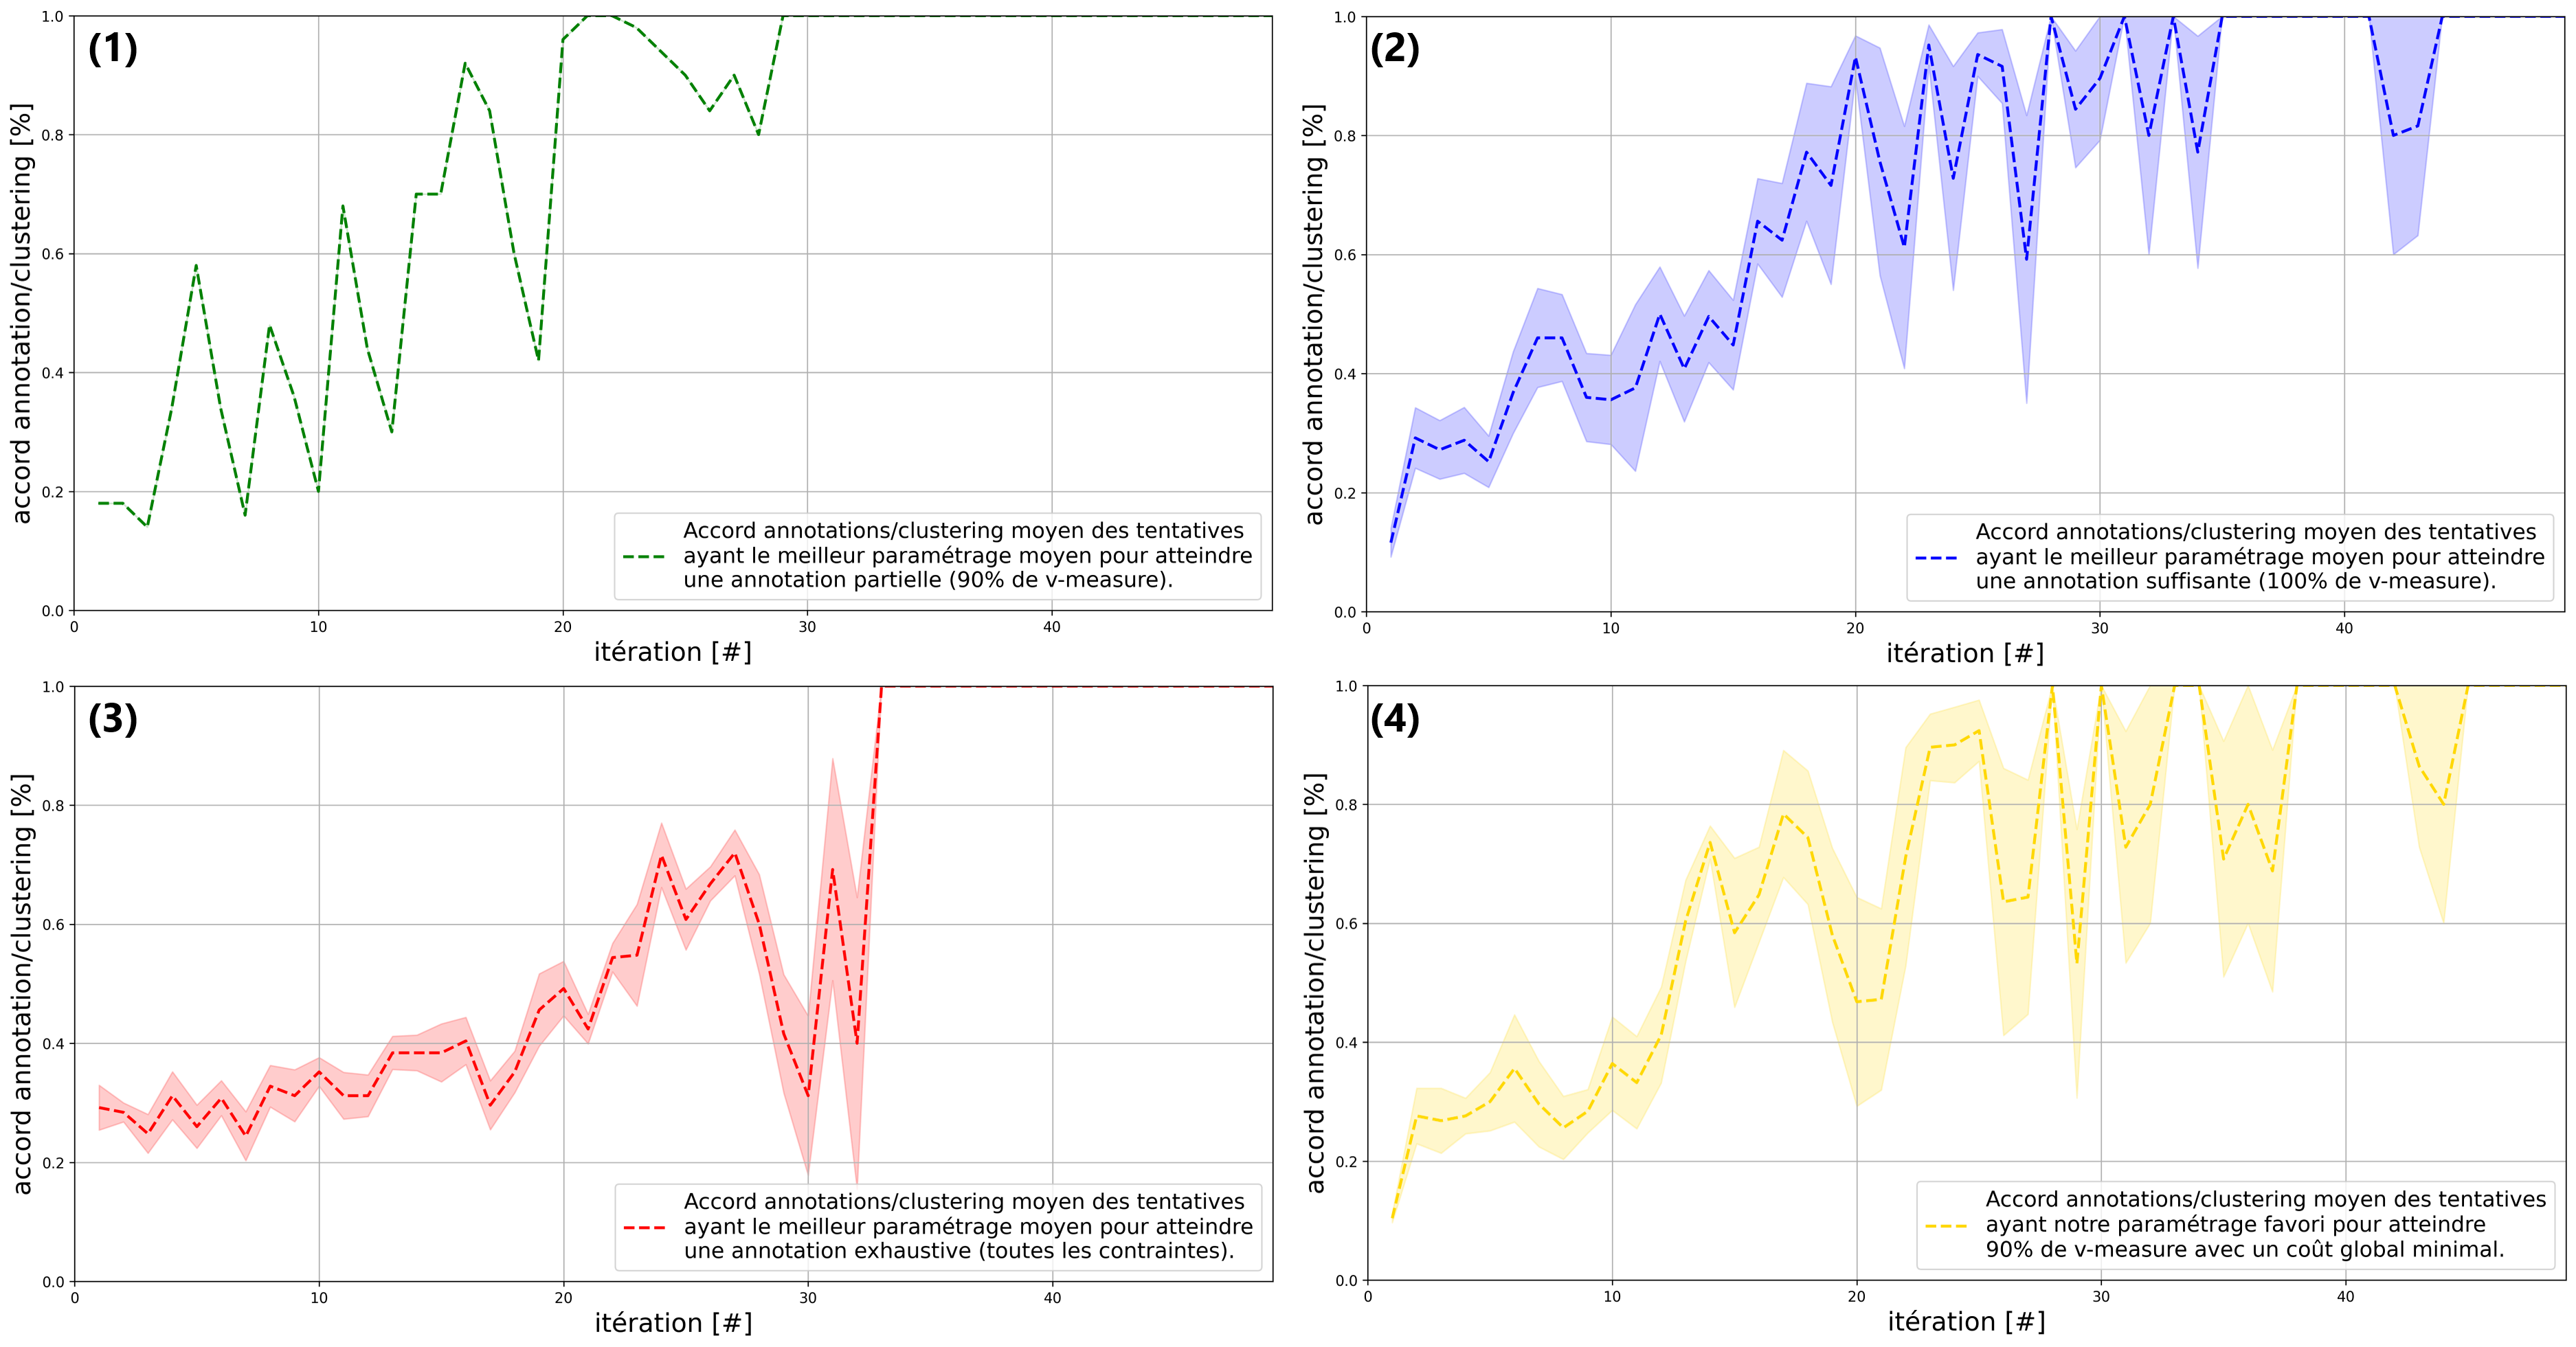
\includegraphics[width=0.95\textwidth]{figures/etude-rentabilite-accord-annotation}
				\caption{Évolution au cours des itérations de l'accord entre l'annotation de contraintes d'un expert et le résultat de \textit{clustering} sur lequel est basé l'échantillonnage de contraintes.
				Ces accords sont exprimés grâce à des lots de $50$ contraintes annotées.
				Les évolutions moyennes de différents paramétrages de la méthode sont exposées :
				\textbf{(1)} meilleur paramétrage moyen pour atteindre une annotation partielle ;
				\textbf{(2)} meilleur paramétrage moyen pour atteindre une annotation suffisante ;
				\textbf{(3)} meilleur paramétrage moyen pour atteindre une annotation exhaustive ;
				et \textbf{(4)} paramétrage favori.
				À titre d'information, les courbes en noir représentent l'évolution de la \texttt{v-measure} entre le \textit{clustering} et la vérité terrain.
				} 
				\label{figure:4.5.1-ETUDE-RENTABILITE-ACCORD-ANNOTATION-CLUSTERING}
			\end{figure}
			
			% Description de la figure : croissance générale.
			À l'aide de la figure, nous pouvons constater une tendance générale à la croissance du score d'accord : l'accord est plutôt faible au début de la méthode (inférieur à $45$\% avant l'itération $15$), puis devient de plus en plus fort (dépassant les $60$\%), et atteint finalement les $100$\% vers l'itération $45$.
			
			% Description de la corrélation entre accord et performance.
			L'analyse de la corrélation \texttt{r} de \textit{Pearson} entre le score d'accord et la performance obtenue avec une vérité terrain donne les résultats suivants :
			\begin{itemize}
				\item $0.49$ sur l’ensemble des tentatives ;
				\item $0.92$ avec le meilleur paramétrage moyen pour atteindre une annotation partielle ;
				\item $0.74$ avec le meilleur paramétrage moyen pour atteindre une annotation suffisante ;
				\item $0.57$ avec le meilleur paramétrage moyen pour atteindre une annotation exhaustive ;
				\item $0.69$ avec les tentatives utilisant le paramétrage favori.
			\end{itemize}
			
			% Description de la figure : croissance instable.
			Cependant, nous pouvons voir que la tendance constatée est saccadée par de nombreux pics pouvant faire perdre ou gagner jusqu'à $40$\% d'accord entre deux itérations.
			Des chutes d'accord peuvent intervenir à des itérations où la similarité du \textit{clustering} avec la vérité terrain est pourtant forte, comme c'est le cas autour des itérations $29$ et $36$ où l'accord chute de plus de $25$\% alors que la \texttt{v-measure} avec la vérité terrain est constamment au dessus de de $95$\%.
			Les autres paramétrages représentés dans \textbf{(1)}, \textbf{(2)} et \textbf{(3)} comportent des tendances similaires (croissance plus au moins rapide, variations soudaines d'accord, chute d'accords pour des \textit{clustering} aux performances élevées, ...).

		%%% Discussion
		\subsubsection{Discussion}
		
			% Rappel de l'objectif : trouver un cas d'arrêt en regardant l'accord entre l'annotation et le clustering.
			Dans cette étude, nous avons analysé l'évolution de l'accord entre les annotations et le partitionnement de données proposé par un \textit{clustering} dans l'espoir de définir un cas d'arrêt de notre méthodologie d'annotation qui soit indépendant d'une vérité terrain pré-établie.
			Cependant, en considérant les résultats obtenus et exposés en \textsc{Figure~\ref{figure:4.5.1-ETUDE-RENTABILITE-ACCORD-ANNOTATION-CLUSTERING}}, ce score d'accord ne semble pas répondre à cette objectif.
			
			% Trop instable pour définir un cas d'arrêt.
			En effet, malgré des score de corrélation passable (moyenne à $0.49$), l'évolution du score d'accord est trop instable pour permettre de définir un cas d'arrêt de la méthode d'annotation : cet accord varie fortement, rendant toute analyse de rentabilité difficile voire impossible.
			En reprenant l'exemple de l'évolution du paramétrage favori (\textsc{Figure~\ref{figure:4.5.1-ETUDE-RENTABILITE-ACCORD-ANNOTATION-CLUSTERING}} \textbf{(4)}), nous ne pouvons pas précisément définir à partir de quelle itération les résultats semblent intéressant car le score d'accord oscille longuement entre $50$\% et $100$\% avec des pics de plus de $25$\% entre deux itérations.
			
			\begin{leftBarAuthorOpinion}
				% Rappel: l'objectif de notre méthode d'annotation est de corriger le plus rapidement un clustering.
				Après réflexion, ce score d'accord est probablement infructueux à cause du fonctionnement même de notre méthode, dont l'objectif est de corriger le partitionnement des données en utilisant un minimum de contraintes.
				En effet, dans le cadre de l'optimisation des paramètres réalisée en \textsc{Section~\ref{section:4.2-HYPOTHESE-EFFICIENCE}}, nous avons retenu dans notre paramétrage favori la sélection des contraintes les plus proches entre deux \textit{clusters} différents (\texttt{samp.closest.diff}) : cette sélection permet ainsi de décrire efficacement l'emplacement des frontières de \textit{clusters}.
				
				% Cet échantillonnage est non supervisé : il y a de nombreuses saccades.
				Or, cet échantillonnage reste une méthode non-supervisée : aux premières itérations, les nouvelles contraintes sélectionnées ont de bonnes chances de mettre en avant une frontière mal positionnée, mais au fur et à mesure que des contraintes s'ajoutent, les nouvelles ont moins de chances de trouver une bordure de \textit{cluster} qui ne soit pas encore caractérisée.
				De ce fait, il se peut que les dernières sélections n'identifient aucune nouvelle frontière, qu'elles se concentrent sur une frontière déjà bien positionnée ou déjà décrite par d'autres contraintes, ou qu'elles nécessite plusieurs itérations pour caractériser une frontière complexe (le comportement des autres méthodes de sélections représentées en \textsc{Figure~\ref{figure:4.5.1-ETUDE-RENTABILITE-ACCORD-ANNOTATION-CLUSTERING}} peut être illustrées par des raisonnements similaires).
				L'ensemble de ces cas de figures peut ainsi expliquer les nombreuses saccades dans l'évolution du score d'accord : tantôt la sélection semble pertinente, tantôt la sélection semble inutile, rendant impossible l'utilisation du score d'accord entre annotation et \textit{clustering} pour définir un cas d'arrêt de la méthode.
			\end{leftBarAuthorOpinion}
			
			% Trop instable pour caratériser une itération.
			Pour aller plus loin, le score d'accord calculé pour une itération ne représente pas non plus les variations dans le score de similitude entre le \textit{clustering} et la vérité terrain.
			En effet, il est rare d'observer des chutes importantes d'accords qui soient accompagnées d'un changement significatif sur l'évolution des performances par rapport à la vérité terrain.
			Il est probable que l'absence de corrélation soit dû à la base de contrainte analysée pour calculer l'accord : les $50$ contraintes annotées peuvent exprimer un désaccord avec le précédent \textit{clustering}, mais ce n'est pas pour autant que l'ajout de ces correctifs ait un impact significatif sur la pertinence globale du partitionnement des données.
			Ce score d'accord n'est donc pas vraiment représentatif de la rentabilité d'une itération.
			
			% Conclusions et suggestion.
			En conclusion, le score d'accord entre l'annotation courante et le \textit{clustering} précédent n'est pas adéquat pour estimer un cas d'arrêt de notre méthode d'annotation, principalement car il est trop instable et qu'il ne représente pas bien les bénéfices obtenus à chaque itération.
	
	%%%
	%%% Subsection 4.5.2: Étude de l'évolution de la différence entre deux \textit{clusterings} consécutifs.
	%%%
	\subsection{Étude de l'évolution de la différence entre deux \textit{clusterings} consécutifs}
	\label{section:4.5.2-ETUDE-RENTABILITE-SIMILARITE-CLUSTERING}
		
		% Objectif de l'expérience.
		Nous venons de conclure que l'analyse de l'accord entre l'annotation et le partitionnement des données ne permet pas d'estimer la rentabilité d'une itération de notre méthode d'annotation.
		Parmi les explications possibles, nous avons mis en cause l'analyse du seul lot de contraintes annotées : en effet, ce n'est pas parce que l'annotation de contraintes est en désaccord avec le précédent partitionnement des données que les correctifs associés auront un impact significatif sur le prochain partitionnement.
		Ainsi, afin d'explorer une piste ayant une vision d'ensemble, nous voulons analyser l'évolution de la différence entre deux \textit{clusterings} successifs : si une itération apporte des correctifs ayant un impact, alors il devrait y avoir des modifications significatives entre ce \textit{clustering} et le suivant.
	
		%%% Protocole expérimental.
		\subsubsection{Protocole expérimental}
			
			% Axiome.
			\begin{leftBarWarning}
				Dans le cadre de cette étude, nous supposons que l'expert métier connaît parfaitement le domaine traité dans ce jeu de données, et qu'il est capable de caractériser sans ambiguïté la similitude entre deux données issues de cet ensemble.
			\end{leftBarWarning}
			
			% Pseudo-code.
			Pour résumer le protocole expérimental que nous décrivons ci-dessous, vous pouvez vous référer au pseudo-code décrit dans \textsc{Algorithme~\ref{algorithm:4.5.1-ETUDE-RENTABILITE-SIMILARITE-CLUSTERING-PROTOCOLE}}.
			
			\begin{algorithm}
				\KwData{jeu de données annotés (vérité terrain)}
				%
				\ForEach{jeux de données à tester}{
					\textbf{initialisation (données)}: récupérer les données et la vérité terrain \;
					\textbf{initialisation (contraintes)}: créer une liste vide de contraintes \;
					\textbf{prétraitement}: supprimer le bruit dans les données avec \texttt{prep.simple} \;
					\textbf{vectorisation}: transformer les données en vecteurs avec \texttt{vect.tfidf} \;
					\textbf{clustering initial}: regrouper les données par similarité avec \texttt{clust.kmeans.cop} \;
					\Repeat{annotation de toutes les contraintes possibles}{
						\textbf{échantillonnage}: sélectionner de nouvelles contraintes à annoter \;
						\textbf{simulation d'annotation}: ajouter des contraintes avec \texttt{samp.closest.diff} \;
						\textbf{clustering}: regrouper les données par similarité avec \texttt{clust.kmeans.cop} \;
						\textbf{estimer rentabilité}: calculer la différence entre les deux derniers \textit{clusterings} \;
					}
				}
				\textbf{analyse 1}: afficher l'évolution de la différence entre deux \textit{clustering} consécutifs \;
				\textbf{analyse 2}: calculer la corrélation entre le score de différence et le score de performance \;
				%
				\KwResult{discussion sur la rentabilité de chaque itération d'après la différence entre \textit{clusterings}}
				%
				\caption{\textit{Description en pseudo-code du protocole expérimental de l'étude de l'évolution de la différence entre deux \textit{clustering} consécutifs.}}
				\label{algorithm:4.5.1-ETUDE-RENTABILITE-SIMILARITE-CLUSTERING-PROTOCOLE}
			\end{algorithm}

			% Détails de l'expérience.
			Nous nous appuyons sur le même protocole que l'expérience précédente (cf. \textsc{Section~\ref{section:4.5.1-ETUDE-RENTABILITE-ACCORD-ANNOTATION-CLUSTERING}}) : nous utilisons comme vérité terrain le jeu de données \texttt{Bank Cards (v1.0.0)}, nous réalisons $5$ tentatives complètes de la méthode du \textit{clustering} interactif utilisant notre paramétrage favori, et nous simulons l'annotation par un expert d'un lot de $50$ contraintes à chaque itération.
			
			% Ajout de la comparaison entre clustering.
			Cependant, au lieu de calculer un score d'accord entre annotation et \textit{clustering}, nous estimons la différence entre le \textit{clustering} précédent et le \textit{clustering} obtenu grâce aux dernières annotations.
			Cette différence entre deux \textit{clustering} $X$ et $Y$ est obtenue par la formule $1-\texttt{v-measure}(X,Y)$ où la \texttt{v-measure} caractérise la ressemblance entre deux partitionnements des données (\cite{rosenberg-hirschberg:2007:vmeasure-conditional-entropybased}).
			Pour nous permettre de discuter de l'utilité de ce score pour prédire la stabilisation du \textit{clustering} et ainsi définir un cas d'arrêt de notre méthodologie d'annotation, nous calculons aussi le score de corrélation entre cette différence et la performance obtenue à l'aide d'une vérité terrain (la corrélation \texttt{r} de \textit{Pearson} (\cite{kirch:2008:pearson-correlation-coefficient}) est utilisée).
			
			% Référence scripts.
			\begin{leftBarInformation}
				Les scripts de l'expérience, réalisés avec des \textit{notebooks} Python (\cite{van-rossum-drake:2009:python-reference-manual}), sont disponibles dans un dossier dédié de~\cite{schild:2021:cognitivefactory-interactiveclusteringcomparativestudy}.
			\end{leftBarInformation}

		%%% Résultats
		\subsubsection{Résultats obtenus}
			
			% Figure.
			La \textsc{Figure~\ref{figure:4.5.2-ETUDE-RENTABILITE-SIMILARITE-CLUSTERING}} représente l'évolution moyenne de la différence entre deux \textit{clusterings} pour les quatre paramétrages mis en avant lors de nos étude.
			Nous concentrons toutefois la discussion sur les résultats obtenus avec le paramétrage favori de notre méthode \textbf{(4)} et utilisons les autres résultats comme points de référence.
			\begin{figure}[!htb]
				\centering
				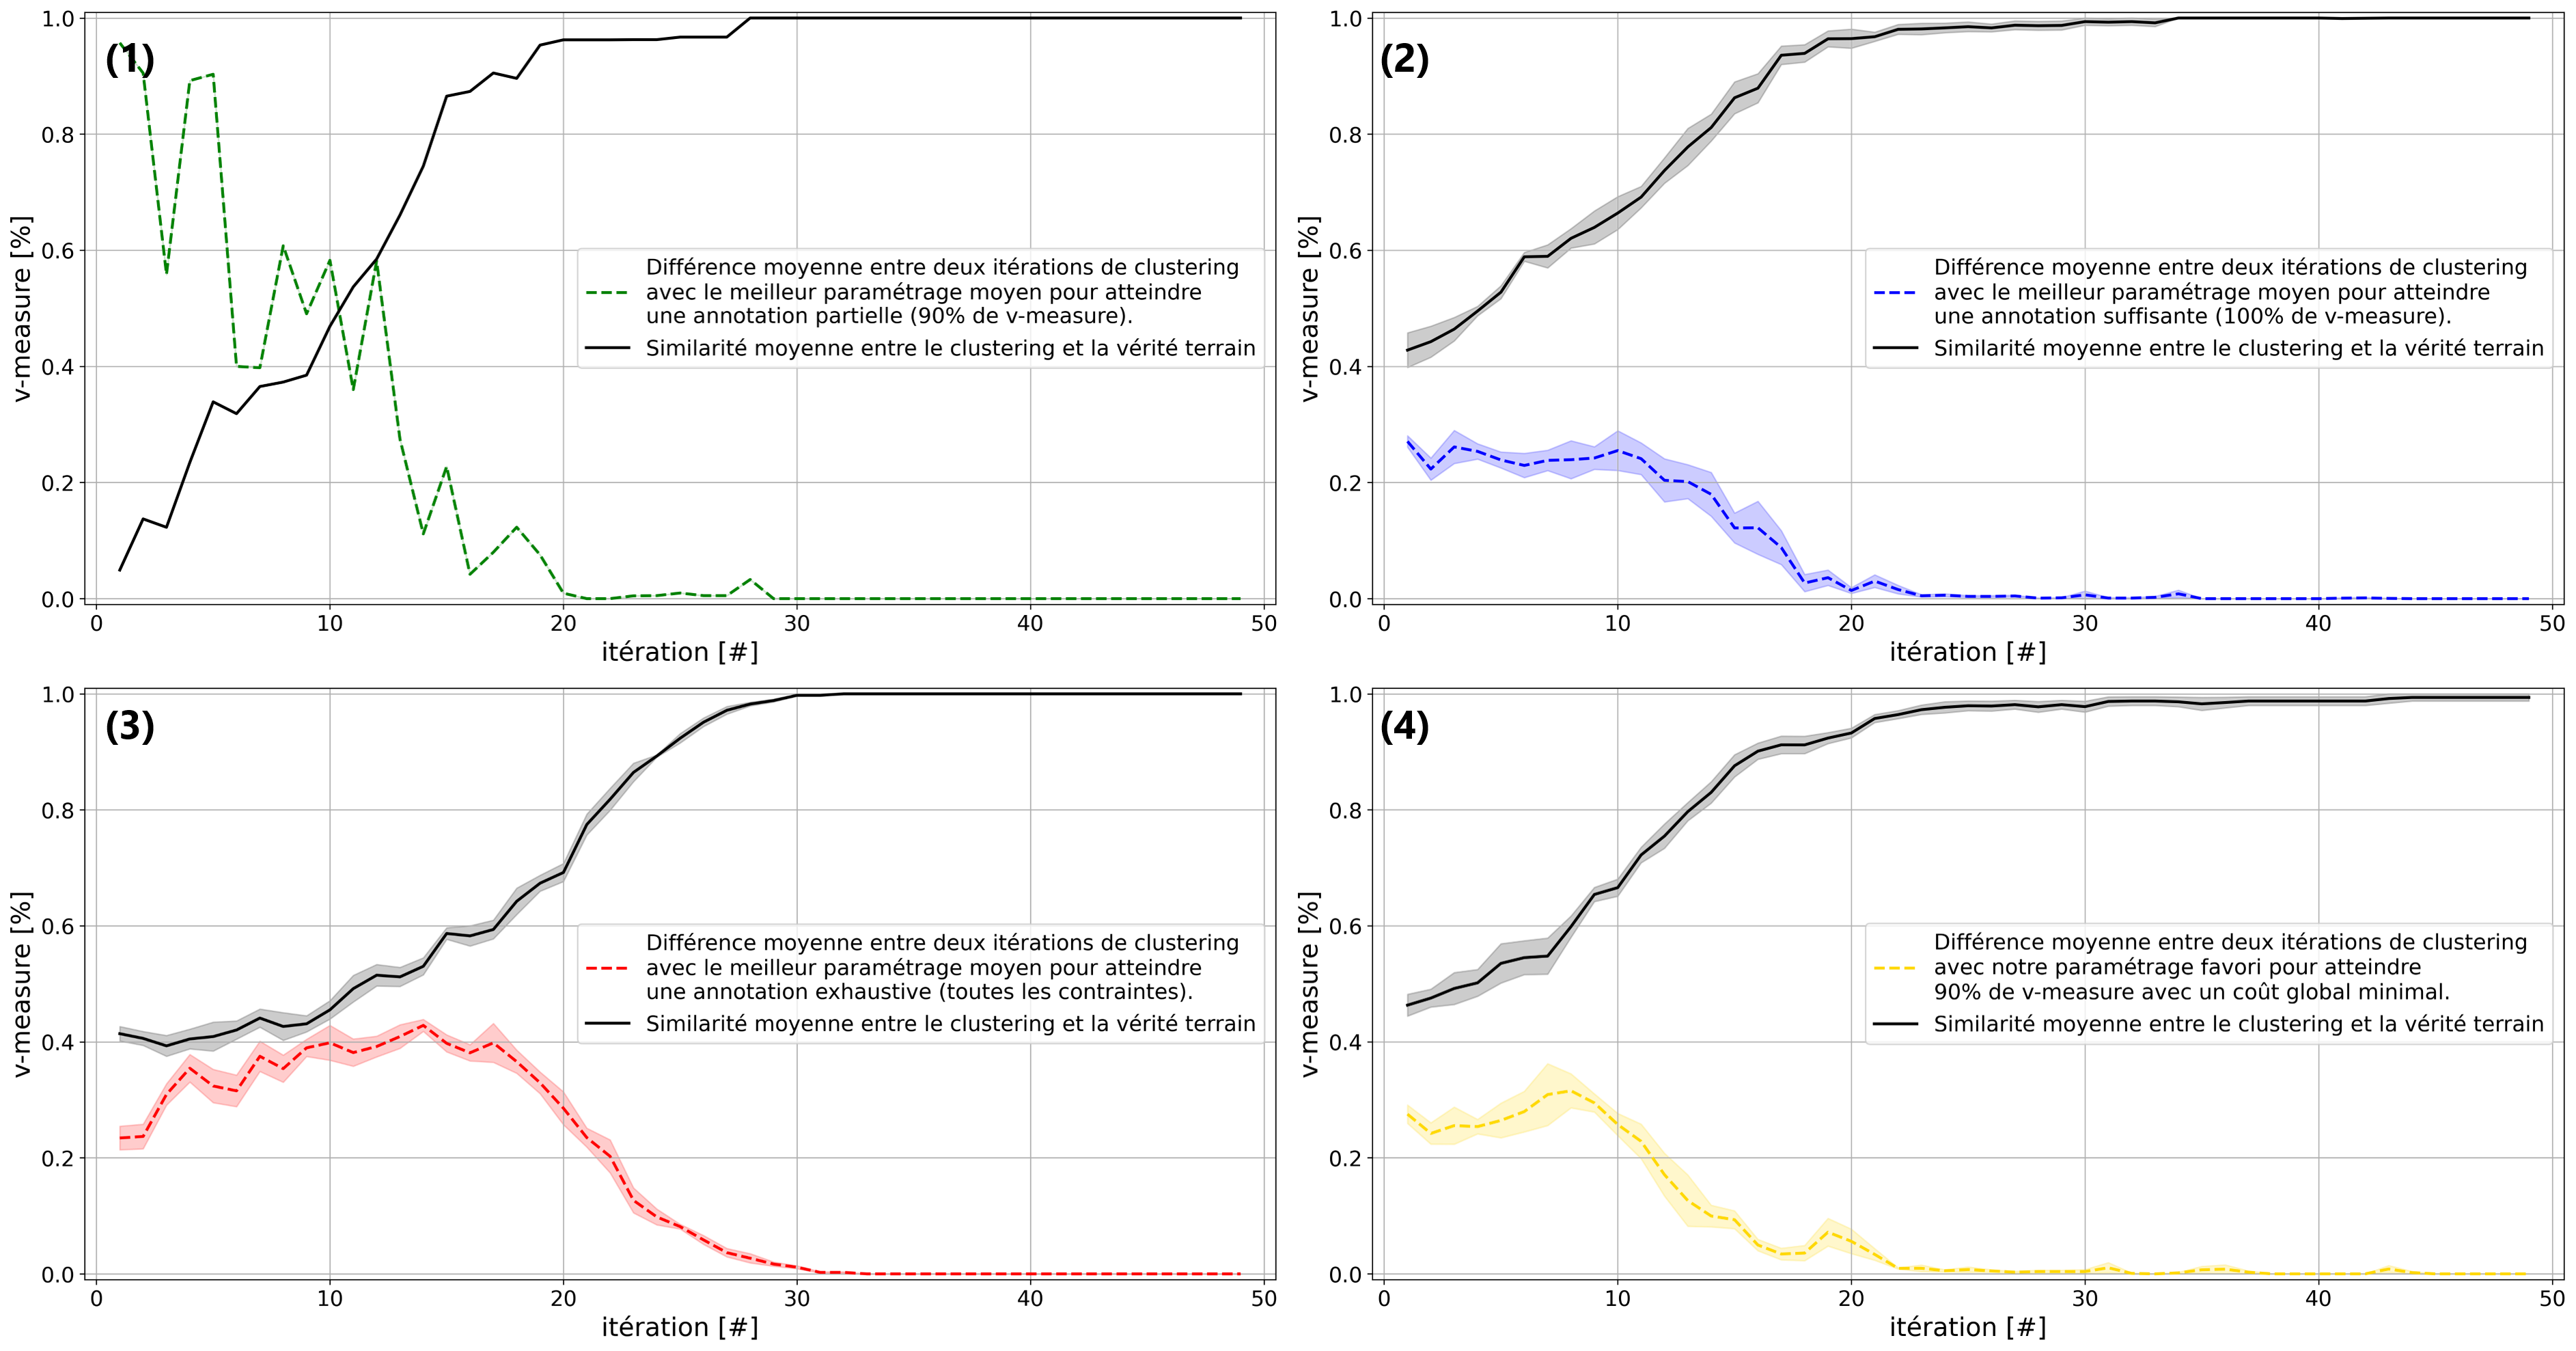
\includegraphics[width=0.95\textwidth]{figures/etude-rentabilite-similarite-clustering}
				\caption{Évolution de la différence de résultats entre deux itérations de \textit{clustering}.
				Les évolutions moyennes de différents paramétrages de la méthode sont exposées :
				\textbf{(1)} meilleur paramétrage moyen pour atteindre une annotation partielle ;
				\textbf{(2)} meilleur paramétrage moyen pour atteindre une annotation suffisante ;
				\textbf{(3)} meilleur paramétrage moyen pour atteindre une annotation exhaustive ;
				et \textbf{(4)} paramétrage favori.
				À titre d'information, les courbes en noir représentent l'évolution de la \texttt{v-measure} entre le \textit{clustering} et la vérité terrain.
				}
				\label{figure:4.5.2-ETUDE-RENTABILITE-SIMILARITE-CLUSTERING}
			\end{figure}
			
			% Description de la figure : décroissance générale.
			À l'aide de la figure, nous pouvons constater une tendance générale à la décroissance vers $0$\% de cette différence.
			Concernant les tentatives utilisant le paramétrage favori \textbf{(4)}, la différence moyenne est initialement comprise entre $25$\% et $35$\% jusqu'à l'itération $10$, elle chute ensuite pour être inférieure à $5$\% après l'itération $20$, et elle termine par oscillant très légèrement ($\pm1$\%) autour de $0$\% jusqu'à la fin des annotations.
			Les tentatives des autres expériences sont similaires à quelques détails : le paramétrage pour atteindre une annotation partielle \textbf{(1)} commence avec des scores de différence très forts et décroît avec avec de nombreux pics ; le paramétrage pour atteindre une annotation exhaustive \textbf{(3)} croît légèrement avant d'entamer sa décroissance.
			
			% Description de la corrélation entre accord et performance.
			L'analyse de la corrélation \texttt{r} de \textit{Pearson} entre le score de différences et la performance obtenue avec une vérité terrain donne les résultats suivants :
			\begin{itemize}
				\item $0.75$ sur l’ensemble des tentatives ;
				\item $0.96$ avec le meilleur paramétrage moyen pour atteindre une annotation partielle ;
				\item $0.92$ avec le meilleur paramétrage moyen pour atteindre une annotation suffisante ;
				\item $0.85$ avec le meilleur paramétrage moyen pour atteindre une annotation exhaustive ;
				\item $0.93$ avec les tentatives utilisant le paramétrage favori.
			\end{itemize}
			Nous pouvons donc affirmer qu'il y une forte corrélation entre ces deux variables.
			
			% Description de la figure : corrélation avec la performance du clustering.
			Nous retrouvons aussi ces corrélations dans la \textsc{Figure~\ref{figure:4.5.2-ETUDE-RENTABILITE-SIMILARITE-CLUSTERING}} :
			\begin{itemize}
				\item un score de \texttt{v-measure} avec la vérité terrain proche de $100$\% est accompagné d'un score de différence proche de $0$\% (après l'itération $20$ pour \textbf{(1)}, après l'itération $20$ pour \textbf{(2)}, après l'itération $30$ pour \textbf{(3)} et après l'itération $22$ pour \textbf{(4)}) ;
				\item une croissance de performance est généralement accompagnée d'un score non nul de différence (voir \textbf{(2)} et \textbf{(4)} entre les itérations $0$ et $20$), et plusieurs pics de performance sont accompagnés de scores forts de différence (particulièrement visible sur \textbf{(1)} vers l'itération $5$ et entre les itérations $10$ et $15$) ;
				\item il est toutefois à noter que l'inverse n'est pas vrai : un score non nul de différence n'accompagne pas forcément une croissance de performance, mais peut simplement caractériser un changement de partitionnement, comme c'est le cas dans \textbf{(3)} entre les itérations $0$ et $10$ où des modifications ont lieu (score de différence non nul) mais où la performance par rapport à la vérité terrain stagne.
			\end{itemize}

		%%% Discussion
		\subsubsection{Discussion}
		
			% Rappel de l'objectif : trouver un cas d'arrêt en regardant l'évolution de la différence entre deux clusterings.
			Dans cette étude, nous avons analysé l'évolution du score de différence entre deux itérations de \textit{clustering} dans l'espoir de définir un cas d'arrêt de notre méthodologie d'annotation qui soit indépendant d'une vérité terrain pré-établie.
			
			% Avantage 1 : Caractérise la rentabilité.
			En considérant les résultats obtenus et exposés en \textsc{Figure~\ref{figure:4.5.2-ETUDE-RENTABILITE-SIMILARITE-CLUSTERING}}, nous pouvons déjà remarquer que ce score de différence permet de représenter efficacement l'impact des correctifs induits par l'annotation.
			En effet, nous constatons une corrélation entre l'évolution de la différence entre deux \textit{clusterings} et l'évolution de la performance du \textit{clustering} par rapport à la vérité terrain à la fois visuelle (courbes inversement proportionnelles) et statistique (score de corrélation de \textit{Pearson} moyen de $0.75$, et scores supérieurs à $0.85$ pour les paramétrages mis en avant).
			
			% Avantage 2 : Permet de définir un cas d'arrêts.
			
			% Attention 1 : Peut ne caractériser qu'un gros changement sans pour autant une amélioration.
			
			% Intérêt 1 : Ne demander de confirmer qu'à certains points d'intérêts
		
			% Remaques.
			\todo[inline]{A REDIGER: Ca montre quand plus rien bouge, fixer un seuil}
			
			% Conclusions et suggestion.
			En conclusion, le score de différences entre deux résultats de \textit{clustering} semble être un bon indicateur de la rentabilité d'une itération, et nous l'utiliserons pour définir un cas d'arrêt de notre méthodologie d'annotation.
			
	%%%
	%%% Subsection 4.5.3: Mise en commun des stratégies d'évaluation de la rentabilité d'une itération de la méthode et définition d'un cas d'arrêt indépendant d'une vérité terrain.
	%%%
	\subsection{Mise en commun des stratégies d'évaluation de la rentabilité d'une itération de la méthode et définition d'un cas d'arrêt indépendant d'une vérité terrain.}
	\label{section:4.5.3-ETUDE-RENTABILITE-MISE-EN-COMMUN}
			
		% Conclusion.
		\begin{leftBarSummary}
			Au cours de cette étude de rentabilité, nous avons pu voir que :
			\begin{itemize}
				\item[\itemko] accords ; % todo
				\item[\itemok] différences ; % todo
				\item[\itemok] cas d'arrêts ; % todo
			\end{itemize}
		\end{leftBarSummary}
		
		% Transition: Vers Simulation d'erreurs.